\documentclass{beamer}
\usepackage{beamerthemeshadow}
\usepackage{verbatim}

\usepackage{lastpage}
\usepackage{xcolor}
\usepackage{pgf}
\usepackage{colortbl}

\newcommand{\bi}{\begin{itemize}}
\newcommand{\ei}{\end{itemize}}
\newcommand{\be}{\begin{enumerate}}
\newcommand{\ee}{\end{enumerate}}
\newcommand{\bd}{\begin{description}}
\newcommand{\ed}{\end{description}}
\newcommand{\prbf}[1]{\textbf{#1}}
\newcommand{\prit}[1]{\textit{#1}}
\newcommand{\beq}{\begin{equation}}
\newcommand{\eeq}{\end{equation}}
\newcommand{\bdm}{\begin{displaymath}}
\newcommand{\edm}{\end{displaymath}}

\newcommand{\ft}[1]{
  \frametitle{\begin{tabular}{p{4.2in}r} \textcolor{white}{#1} & \small{\insertframenumber / \inserttotalframenumber} \end{tabular}}
  \setbeamercovered{transparent=18}
}

\newcommand{\stepinv}{\setbeamercovered{invisible}}
\newcommand{\stopinv}{\setbeamercovered{transparent=18}}
\newcommand{\uncoverinv}[1]
{
  \setbeamercovered{invisible}
  \uncover<+->{#1}
  \setbeamercovered{transparent=18}
}
\newcommand{\ans}[1]{\textcolor{blue}{#1}}
\newcommand{\ansinv}[1]
{
  \setbeamercovered{invisible}
  \uncover<+->{\textcolor{blue}{#1}}
  \setbeamercovered{transparent=18}
}
\newcommand{\setinv}{\setbeamercovered{invisible}}
\newcommand{\setvis}{\setbeamercovered{transparent=18}}
\newcommand{\centerpic}[2]
{
  \begin{center}
  \includegraphics[#1]{#2}
  \end{center}
}
\newcommand{\h}[1]{\hat{#1}}
\newcommand{\ds}{\displaystyle}

%\definecolor{light}{rgb}{1.0,0.33,0.33}
\definecolor{light}{rgb}{1.0,0.5,0.5}
\newcommand{\hl}[1]{\alt<#1>{\rowcolor{light}\hspace*{-2.1pt}} {\hspace*{-2.1pt}} }

\definecolor{mycolor}{rgb}{0.6,0.0,0.0}
\usecolortheme[named=mycolor]{structure}

\title{Regime Switching, Learning, and the Great Moderation}
\author[UW-La Crosse Economics Department Visit. January 2009.]{James Murray\\Dahl School of Business\\Viterbo University}
\date{January 23, 2009}

\begin{document}

\frame{\titlepage}
\setcounter{framenumber}{0}

\section{Introduction}
\subsection{Purpose}
\frame
{
  \ft{Time Varying Volatility}
  \begin{center}
    \begin{tabular}{cc}
      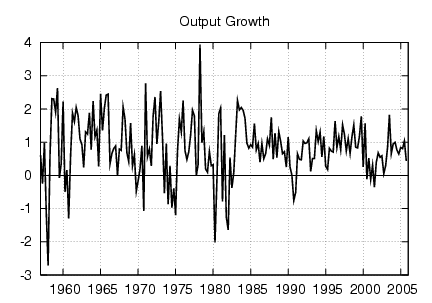
\includegraphics[scale=0.35]{plots/ydata.png} &
      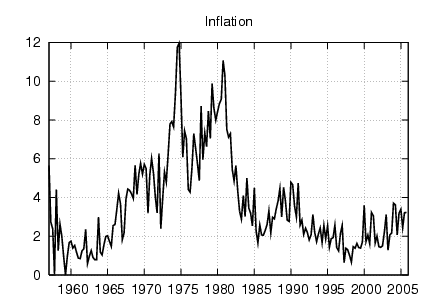
\includegraphics[scale=0.35]{plots/pidata.png} \\
    \end{tabular}
  \end{center}
}

\frame
{
  \ft{Purpose}
  \bi
  \item<+-> How much does ``bad luck'' explain changing volatility when adaptive expectations react to suspicions of structural changes.
  \item<+-> \textbf{Great Moderation:} seemingly permanent reduction in macroeconomic volatility since approximately 1982.
  \item<+-> \textbf{Bad Luck:} volatile periods were hit with bad shocks.
  \item<+-> \textbf{Adaptive Expectations:} 
    \bi
    \item<+-> Least squares learning - agents run least-squares regressions
    \item<+-> Predict output and inflation using lagged output, inflation, and interest rates as explanatory variables.
    \ei
  \ei
}

\subsection{Reasons for the Great Moderation}
\frame
{
  \ft{Great Moderation Explanations}
  \bi
  \item<+->Good vs. bad policy.
    \bi
    \item<+->Lubik and Schorfheide (2004): find monetary policy was destabilizing pre-Volker.
    \item<+->Milani (2005): accounting for learning, little evidence of a change in monetary policy.
    \ei
  \item<+->Bad luck
    \bi
    \item<+->Sims and Zha (2006): evidence points in favor of bad shocks.
    \item<+->Bullard and Singh (2007): bad luck + Bayesian learning.
    \ei
  \item<+->Learning
    \bi
    \item<+->It is possible for learning \textit{alone} to generate time-varying volatility.
    \item<+->Primiceri (2005), Oraphnides and Williams (2005): Monetary authority was optimizing, but mis-informed.
    \ei
  \ei
}

\subsection{Dynamic Gain Learning}
\frame
{
  \ft{Learning Gain}
    \bi
    \item<+-> Learning gain: how much weight is given to the last (most recent) observation.
    \item<+-> Decreasing learning gain
      \bi
      \item<+-> Ordinary least squares - learning gain = 1/n.
      \item<+-> As time progresses, sample size increases, learning gain decreases.
      \item<+-> Implies agents do not suspect structural change.
      \item<+-> Learning dynamics disappear over time.
      \ei
    \item<+-> Constant learning gain
      \bi
      \item<+-> Gives more weight to most recent observations - weight declines geometrically with time.
      \item<+-> Agents have constant suspicion of structural change.
      \item<+-> Learning dynamics persist in the long run.
      \ei
    \ei
}

\frame
{
  \ft{Dynamic Learning Gain}
  \bi
  \item<+-> Dynamic Gain Learning: agents endogenously switch between decreasing and constant learning gain.
    \bi
    \item<+-> Agents use decreasing gain unless forecast errors exceed a threshold.
    \item<+-> Threshold = historical average absolute value forecast error.
    \item<+-> Agents only suspect structural change when forecast errors are exceptionally high.
    \ei
  \item<+-> Milani (2007): generates ARCH time-varying volatility
  \item<+-> Marcet and Nicolini (2003): recurrent hyperinflations.
  \ei
}

\subsection{Approach}
\frame
{
  \ft{Approach}
  \bi
  \item<+-> Use a standard, commonly estimated monetary model: New Keynesian Model.
    \bi
    \item<+-> Three equation model with optimizing consumers, sticky prices, monetary policy.
    \item<+-> Stochastic shocks: demand shock, cost-push shock, monetary policy shock.
    \ei
  \item<+-> Augment the model with dynamic gain learning.
  \item<+-> Also estimate model under RE and constant gain learning.
  \item<+-> Augment the model with Markov switching process for volatility.
    \bi
    \item<+-> Volatile regime: shocks have high variances.
    \item<+-> Less volatile regime: shocks have relatively lower variances.
    \item<+-> Economy switches between these two regimes by luck.
    \ei
  \ei
}

\frame
{
  \ft{Questions}
    \bi
    \item<+-> Does the dynamic gain model predict a lower likelihood economy was in volatile regime?
      \bi
      \item<+-> Spoiler: No.
      \ei
    \item<+-> When is the economy in the volatile regime?
      \bi
      \item<+-> Spoiler: All models predict dates surrounding NBER recessions of 1970s.
      \ei
    \item<+-> Does the dynamic gain model predict lower variances for volatile regime shocks?
      \bi
      \item<+-> Spoiler: Yes.
      \ei
    \item<+-> When are agents using larger learning gain?
      \bi
      \item<+-> Spoiler: During most of the 1970s.
      \ei
    \item<+-> What expectations mechanism fits the data best?
      \bi
      \item<+-> Spoiler: Rational expectations, constant gain learning, decreasing learning have nearly identical fit.
      \ei
  \ei
}

\section{New Keynesian Model}
\subsection{Consumer Behavior}
\frame
{
  \ft{New Keynesian Model: Optimal Consumer Behavior}
  \bi
  \item<+-> Consumers maximize net present value of lifetime utility, subject to their budget constraint.
  \item<+-> As the real interest rate increases, consumers decide to save more, consume less.
  \item<+-> The size of this effect depends on the \textbf{intertemporal elasticity of substitution}, estimated in paper.
  \item<+-> As the expected inflation rate rises, expected real interest rate falls.
  \item<+-> Habit formation: current consumption (current utility) depends on past consumption.
  \item<+-> \textbf{Degree of habit formation} is between 0 and 1, estimated in paper.
  \item<+-> Consumption subject to a \textit{demand shock}.
  \ei
}

\subsection{Producer Behavior}
\frame
{
  \ft{New Keynesian Model: Optimal Producer Behavior}
  \bi
  \item<+-> Monopolistically competitive firms.
  \item<+-> Exogenously sticky prices: it takes firms an uncertain amount time to appropriately adjust prices to maximize profits.
  \item<+-> Sticky prices enable monetary policy to have real effects on short-run output.
  \item<+-> Price indexation: when firms cannot re-optimize prices, they raise their prices by the past period's rate of inflation.
  \item<+-> \textbf{Degree of indexation} is between 0 and 1, estimated in the paper.
  \item<+-> Inflation subject to a \textit{cost shock}.
  \ei
}

\subsection{Monetary Policy}
\frame
{
  \ft{New Keynesian Model: Monetary Policy}
  \bi
  \item<+-> Fed adjusts Federal Funds Rate according to Taylor (1993) rule.
  \item<+-> Federal funds rate in response to:
    \bi
    \item<+-> output gap
    \item<+-> inflation rate
    \item<+-> past federal funds rate (Fed makes smooth adjustments)
    \ei
  \item<+-> The response to these variables are estimated in paper.
  \item<+-> Federal funds rate is subject to a \textit{monetary policy shock}.
  \ei
}

\section{Estimation Results}
\subsection{Estimation Procedure}
\frame {
  \ft{Estimation Procedure}
  \bi
  \item<+-> Maximum Likelihood
    \bi
    \item<+-> Use Kim and Nelson (1999) method.
    \ei
  \item<+-> Quarterly data from 1960:Q1 through 2008:Q1
    \bi
    \item<+-> Output gap: measured by Congressional Budget Office.
    \item<+-> CPI inflation rate.
    \item<+-> Federal funds rate.
    \ei
  \item<+-> Pre-sample period to initialize expectations: 1954:Q3 - 1959:Q4.
  \item<+-> Expectations are initialized to pre-sample VAR(1) results.
  \ei
}

\subsection{Parameter Estimates}
\frame {
  \ft{Parameter Estimates}
\tiny
  \begin{center}
    \begin{tabular}{cl|l|l|l}\hline
 & Parameter & Rational Expectations & Dynamic Gain & Constant Gain \\ \hline
\hl{4}
$\sigma_{n,L}$ & Nat. Rate (Low)& 0.1768 (0.3720) & 0.0454 (0.0217) & 0.0931 (0.0572) \\ 
\hl{5}
$\sigma_{u,L}$ & Cost Push (Low)& 0.0023 (0.0001) & 0.0045 (0.0004) & 0.0042 (0.0001) \\ 
\hl{6}
$\sigma_{r,L}$ & MP Shock (Low)& 0.0013 (0.0001) & 0.0012 (0.0000) & 0.0012 (0.0000) \\ 
\hl{4}
$\sigma_{n,H}$ & Nat. Rate (High)& 0.4295 (0.9056) & 0.0966 (0.0485) & 0.1794 (0.1144) \\ 
\hl{5}
$\sigma_{u,H}$ & Cost Push (High)& 0.0044 (0.0004) & 0.0092 (0.0010) & 0.0085 (0.0005) \\ 
\hl{6}
$\sigma_{r,H}$ & MP Shock (High)& 0.0070 (0.0005) & 0.0064 (0.0003) & 0.0056 (0.0002) \\ 
\hl{3}
$p_{L}$ & P(Remain Low) & 0.9609 (0.0224) & 0.9724 (0.0097) & 0.9780 (0.0109) \\ 
\hl{3}
$p_{H}$ & P(Remain High) & 0.8099 (0.0578) & 0.8924 (0.0264) & 0.9412 (0.0159) \\ 
\hl{2}
$g$ & Learning Gain & -- & 0.0045 (0.0007) & 0.0000 (0.0018) \\ \hline 
\end{tabular}
\end{center}
\normalsize
\only<1>{\vspace*{1.0pc}}
\only<2>{\textcolor{mycolor}{Expectations are not adaptive.}}
\only<3>{\textcolor{mycolor}{Regimes are highly persistent.}}
\only<4>{\textcolor{mycolor}{Learning predicts smaller variances of the natural rate shock.}}
\only<5-6>{\textcolor{mycolor}{Variances of cost push and monetary shock are similar.}}
}

\subsection{Regime-Switching Volatility}
\frame
{
  \ft{Regime-Switching Volatility}
  \begin{center}
    Rational Expectations\\
    Probability Economy is in the Volatile Regime\\
    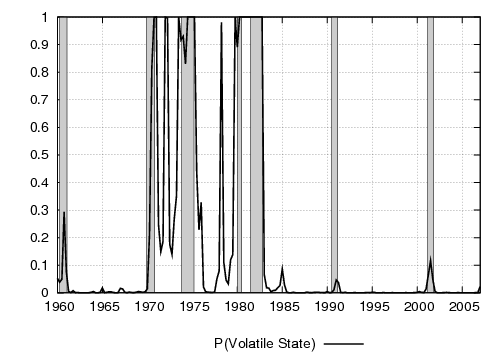
\includegraphics[scale=0.4]{results_re/states_sm.png} \\
    Expected 7.77 volatile years
  \end{center}
}

\frame
{
  \ft{Regime-Switching Volatility}
  \begin{center}
    Constant Gain Learning\\
    Probability Economy is in the Volatile Regime\\
    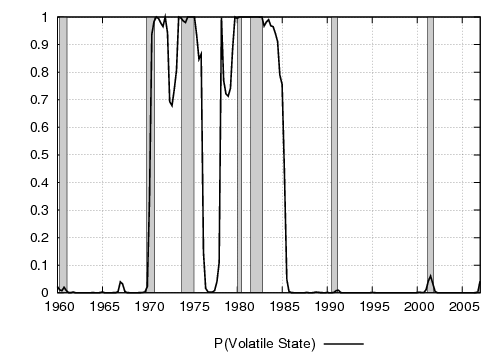
\includegraphics[scale=0.4]{results_cg_wlsinit/states_sm.png} \\
    Expected 12.26 volatile years
  \end{center}
}

\frame
{
  \ft{Regime-Switching Volatility}
  \begin{center}
    Dynamic Gain Learning\\
    Probability Economy is in the Volatile Regime\\
    and Evolution of the Learning Gain\\
    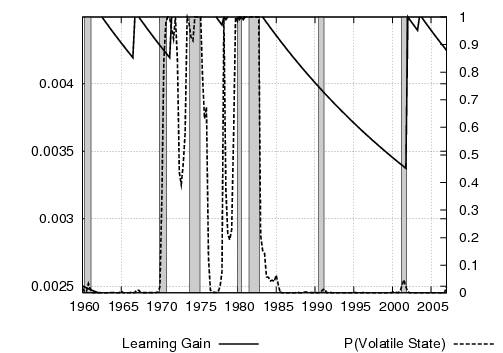
\includegraphics[scale=0.4]{results_dg8_wlsinit/states_sm.png} \\
    Expected 9.17 volatile years
  \end{center}
}

\subsection{Forecast Errors}

\frame
{
  \ft{Forecast Errors Comparison}
\tiny
  \begin{center}
\begin{tabular}{|l|c|c|c|}\hline
 & Rational Expectations & Dynamic Gain & Constant Gain \\ \hline 
RMSE Output Gap & 3.12 & 3.13 & 3.18 \\ 
RMSE Inflation & 4.41 & 4.69 & 4.69 \\ 
RMSE Federal Funds Rate & 5.01 & 5.05 & 5.09 \\ \hline 
AR(1) Output Variance & 0.0904 (0.0730) & 0.1715 (0.0722) & 0.1240 (0.0728) \\ 
AR(1) Inflation Variance & 0.1760 (0.0716) & 0.1364 (0.0699) & 0.1073 (0.0653) \\ 
AR(1) Fed Funds Variance & 0.3851 (0.0670) & 0.3798 (0.0659) & 0.3798 (0.0636) \\ \hline 
\end{tabular}
\end{center}
\normalsize
\bi
\item<+-> Rational Expectations actually (very slightly) fits data better than learning models.
\item<+-> All models show some persistence in volatility of forecast errors.
\item<+-> Models especially fail to explain changing volatility of the federal funds rate.
\ei
}

\frame {
  \ft{Forecast Errors: Output Gap}
  \begin{tabular}{ccc}
  Rational Exp. (1.0) & Constant Gain (0.86) & Dynamic Gain (0.82) \\
  \includegraphics[scale=0.18]{../badluck/results_re/output_err.png} &
  \includegraphics[scale=0.18]{../badluck/results_cg_wlsinit/output_err.png}  &
  \includegraphics[scale=0.18]{../badluck/results_dg8_wlsinit/output_err.png} \\
  \end{tabular}

  \bi
  \item (Correlation with Rational Expectations)
  \item All models made similar errors
  \item Most volatile during recessions in 1970s, early 1980s
  \ei
}

\frame {
  \ft{Forecast Errors: Inflation}
  \begin{tabular}{ccc}
  Rational Exp. (1.0) & Constant Gain (0.85) & Dynamic Gain (0.80) \\
  \includegraphics[scale=0.18]{../badluck/results_re/inflation_err.png} &
  \includegraphics[scale=0.18]{../badluck/results_cg_wlsinit/inflation_err.png}  &
  \includegraphics[scale=0.18]{../badluck/results_dg8_wlsinit/inflation_err.png} \\
  \end{tabular}

  \bi
  \item (Correlation with Rational Expectations)
  \item All models made similar errors.
  \item Most volatile during recessions in 1970s, early 1980s.
  \ei
}

\frame {
  \ft{Forecast Errors: Federal Funds Rate}
  \begin{tabular}{ccc}
  Rational Exp. (1.0) & Constant Gain (0.99) & Dynamic Gain (0.99) \\
  \includegraphics[scale=0.18]{../badluck/results_re/fedfunds_err.png} &
  \includegraphics[scale=0.18]{../badluck/results_cg_wlsinit/fedfunds_err.png}  &
  \includegraphics[scale=0.18]{../badluck/results_dg8_wlsinit/fedfunds_err.png} \\
  \end{tabular}

  \bi
  \item (Correlation with Rational Expectations)
  \item Essentially identical errors.
  \item Do not explain change in policy in early 1980s.
  \ei
}

\section{}
\subsection{Conclusion}
\frame
{
  \ft{Conclusions}
  \bi
  \item<+-> When allowing for regime-switching volatility, there is little evidence of adaptive expectations.
  \item<+-> Constant gain learning and dynamic gain learning both produce less volatility for the natural rate shock.
  \item<+-> Learning frameworks actually deliver a higher prediction for the time spent in volatile regime.
  \item<+-> All models make similar forecast errors at similar points in sample.
  \item<+-> Rational expectations model actually yields smallest in-sample MSE.
  \ei
}

\section{Research Program}
\frame
{
  \ft{Research Program}
  \bi
  \item<+-> Rational expectations fails to deliver widely cited behavior of expectations.
  \item<+-> New Keynesian model fails to deliver common features of data:  persistence, volatility clustering, great moderation.
  \item<+-> My current papers: Empirical Examination of Learning.
    \bi
    \item<+-> Examine importance of choosing initial expectations.
    \item<+-> Consider role of investment / capital accumulation.
    \item<+-> Dynamic Gain.
    \ei
  \item<+-> Future - Consider more dynamic expectations.
    \bi
    \item<+-> Branch (2004): Heterogeneous expectations.
    \item<+-> Henzel (2008): Time-varying monetary policy - signal extraction learning.
    \item<+-> Bullard, Evans, Honkapohja (2007): Near-rational exuberance. 
    \item<+-> Include survey forecasts (Michigan survey, Survey of Professional Forecasters).
    \ei
  \ei
}

\frame
{
  \ft{Other Research Projects}
  \bi
  \item<+-> Scholarship of teaching and learning
    \bi
    \item<+-> Does living in a dormitory improve student performance?
    \item<+-> Through what channels?
    \item<+-> Account for endogeneity.
    \ei
  \item<+-> Policy to reduce spread of AIDS and risky behavior in Africa.
    \bi
    \item<+-> Developing a model of overlapping generations, risky behavior, short life expectancy, and life-insurance.
    \item<+-> Calibrate model and ask if life-insurance plan is feasible.
    \ei
  \ei
}

\end{document}

